\documentclass[11pt,a4paper,twoside]{article}

%%%%%%%%%%%%%%%%%%%%%%%%%%
%	Package imports
%%%%%%%%%%%%%%%%%%%%%%%%%%

% Text and Font
\usepackage[T1]{fontenc}
\usepackage[applemac]{inputenc}

% Lists
\usepackage{enumitem}
\setlist{noitemsep}

% Mathematics

\usepackage{amsmath}
\usepackage{amssymb}
\usepackage{amsthm}
\usepackage{mathtools}
\usepackage{algorithm}
\usepackage{algpseudocode}
\usepackage{physics}
\usepackage{bbm}
%\usepackage{unicode-math}
%\usepackage{mathspec}% for identity symbol

%%%%
% copied from baayen report
\usepackage{array}
%
\usepackage{colortbl}
\usepackage{tabularx}
%
\usepackage{lipsum}
\usepackage{setspace}
% adjust lines in table
\usepackage{booktabs}
%\usepackage[usenames]{color}
\definecolor{tblhead}{RGB}{242, 242, 242}
\usepackage{xcolor}
\newcommand{\mathds}[1]{\text{\usefont{U}{dsrom}{m}{n}#1}}
% end copied from baayen report
% Tables
\usepackage{booktabs}

% Graphics and color
\usepackage{graphicx}
\usepackage{xcolor}

% References and Bibliography
\usepackage{url}
\usepackage{hyperref}
\hypersetup{
  colorlinks,
  linkcolor={black},
  citecolor={blue!50!black},
  urlcolor={blue!50!black}
}
\usepackage{cleveref}
\usepackage[numbered]{bookmark} % Fixes false PDF table of contents
\usepackage{natbib}
\setcitestyle{numbers,sort&compress,square,comma}
\usepackage{bibentry}
\nobibliography*

% Sizing and Dimensions
\setlength{\voffset}{-28.4mm}
\setlength{\hoffset}{-1in}
\setlength{\topmargin}{20mm}
\setlength{\oddsidemargin}{25mm}
\setlength{\evensidemargin}{25mm}
\setlength{\textwidth}{160mm}

% Text
\usepackage[parfill]{parskip} % Remove paragraph indentation
\setlength{\textheight}{235mm}
\setlength{\footskip}{20mm}
\setlength{\headsep}{50pt}
\setlength{\headheight}{0pt}

%%%%%%%%%%%%%%%%%%%%%%%%%%
%	Style and command definitions
%%%%%%%%%%%%%%%%%%%%%%%%%%

%Theorem-type environments
\newtheoremstyle{thmbreak}
  {}
  {}
  {\itshape}
  {}
  {\bfseries}
  {}
  {\newline}
  {}
\theoremstyle{thmbreak}
\newtheorem{Theorem}{Theorem}
\numberwithin{Theorem}{subsection}
\newtheorem{Proposition}[Theorem]{Proposition}
\newtheorem{Corollary}[Theorem]{Corollary}
\newtheorem{Lemma}[Theorem]{Lemma}
\newtheoremstyle{defbreak}
  {}
  {}
  {}
  {}
  {\bfseries}
  {}
  {\newline}
  {}
\theoremstyle{defbreak}
\newtheorem{Definition}[Theorem]{Definition}
\theoremstyle{remark}
\newtheorem{Remark}[Theorem]{Remark}
\theoremstyle{remark}
\newtheorem{Example}[Theorem]{Example}

\usepackage{hyperref}
\usepackage{cleveref}



%%%%%%%%%%%%%%%%%%%%%%%%%%
%	Document Body
%%%%%%%%%%%%%%%%%%%%%%%%%%
\begin{document}

\pagestyle{empty}

%%%%%%%%%%%%%%%%%%%%%%%%%%%%%%%%%%%%%%%%%%%%%%%%%%%%%%%
%%% Title page
%%%%%%%%%%%%%%%%%%%%%%%%%%%%%%%%%%%%%%%%%%%%%%%%%%%%%%

\begin{titlepage}

	%%%%%%%%%%%%%%%%%%% LOGO  %%%%%%%%%%%%%%%%%%%%%%%%%%%%
	\begin{figure}
		\begin{center}
			
\includegraphics[scale=.7]{img/hku-logo.png} % rot
			%\includegraphics[scale=.3]{img/logo_sw.pdf} % schwarz
		\end{center}
	\end{figure}
	%%%%%%%%%%%%%%%%%%%%%%%%%%%%%%%%%%%%%%%%%%%%%%%%%%%%%%%%




\begin{center}
  {\LARGE The University of Hong Kong}\\
  {\large Department of Computer Science\\
   
    \vspace*{2cm}
  {\huge Final Project\\[1.5cm]}}
%	{\Large\bf Probabilistic modelling of  Infectious Diseases\\[1.5cm]}
    {\Large\bf Text Classification and Information Retrieval}\\ [0.2cm]
    {\large   Automatic Recognition of Emotions from Recorded Speech Data.\\[1.5cm]}
  {\large Hanna Dettki}\\
  \href{mailto:hanna.dettki@student.uni-tuebingen.de}{hanna.dettki@student.uni-tuebingen.de}



\end{center}

\vfill
Lecturer: Professor Dr. Yu Lequan\\


UID: 3035960651, 
\href{mailto:u3596065@connect.hku.hk}{u3596065@connect.hku.hk}

Date: \today

\end{titlepage}

%%%%%%%%%%%%%%%%%%%%%%%%%%%%%%%%%%%%%%%%%%%%%%%%%%%%%%%%%%%%%%%%%%%%%%%%%%%%%%%%%%%%%%%%%%%%%%%%%%%%%%%%%%%%
%%%%%%%%%%%%%%%%%%%%%%%%%%%%%%%%%%%%%%%%%%%%%%%%%%%%%%%%%%%%%%%%%%%%%%%%%%%%%%%%%%%%%%%%%%%%%%%%%%%%%%%%%%%%


%%%%%%%%%%%%%%%%%%%%%%%%%%%%%%%%%%%%%%%%%%%%%%%%%%%%%%%%%%%%%%%%%%%%%%%%%%%%%%%%%%%%%%%%%%%%%%%%%%%%%%%%%%%%
%%% Table of contents
\setcounter{tocdepth}{3}
\tableofcontents
\newpage

% Page numbering restarts here
\pagenumbering{arabic}
\pagestyle{headings}


%%%%%%%%%%%%%%%%%%%%%%%%%%%%%%%%%%%%%%%%%%%%%%%%%%%%%%%%%%%%%%%%%%%%%%%%%%%%%%%%%%%%%%%%%%%%%%%%%%%%%%%%%%%
%%%%%%%%%%%%%%%%%%%%%%%%%%%%%%%%%%%%%%%%%%%%%%%%%%%%%%%%%%%%%%%%%%%%%%%%%%%%%%%%%%%%%%%%%%%%%%%%%%%%%%%%%%%%
\begin{abstract}
Natural intercommunication between humans and computers is a key  aspect to be achieved in the research of  natural language processing (NLP).
In order to not only have the machine understand verbal content, but also more subtle signals that any human being would readily react to, inferring emotions from spoken speech in real-time therefore is a fundamental ability for the machine to have.

In this work, two machine learning approaches
are evaluated against the task of classifying purely acoustic data as one out of eight possible emotions, namely a Convolutional Neural Network (CNN) and a  Support Vector Machine (SVM). 
It is shown that the SVM significantly outperforms  the Deep Learning approach while only taking the most relevant frequency bands into account.
Although the latter one is not provided with any temporal context, it predicts emotions on a test set with an  accuracy of 63.89\% and with an accuracy of 97.05\% on the training set.
\end{abstract}

\section{Introduction}
Aiming for  natural human computer interaction, automatic emotion recognition from speech is a fundamental prerequisite.
Automatic speech recognition (ASR) and human auditory comprehension is at the bottom of automatic emotion recognition from speech. 
It is therefore beneficial to have a good understanding of speech perception and language processing in humans as well as the neurophysiology of the auditory system.

 
The overall research question underlying various scientists' research in this field  is still to gather an understanding of how  a speaker's motor gestures  are transformed to sounds and how those sounds are mapped onto meaning in the comprehension of spoken language \cite{moore2008introduction}.  
Despite ASR being a field of research, which is approached by different disciplines of research and there therefore encapsulates a plethora of models such as the classical linguistic one, the cognitive, or engineering one \cite{shafaei2018wide}, there has been little interaction between those groups according to Moore \cite{moore2008introduction}.
While human computer interaction (HCI) control  mechanisms previously have relied only on textual or display-based control mechanisms, allowing only the speaker's word-based requests,
more intuitive mechanisms are being implemented, exploiting the speaker's  voice, gestures, and mimic. 
The latter ones reveal much more information on the speaker's intentions since more context information is 
 taken into account, such as emotions.

 Speech provides a high density of information of which humans percept categories such as \textit{phones} (physical properties of speech sounds) and \textit{phonemes} (systematic organization of sounds). 
Consequently, it seems to be important to extract such features and map their acoustic properties to emotions in order to provide machines with a better understanding of the human speech.
However, in this work, a machine learning approach which only takes the most relevant frequencies into account while losing the temporal context, turns out to work pretty well.



\section{Related Work}

\subsection{Acoustic Properties in Speech}
Speech provides a high range and density of acoustical information of which the science of phonetics is concerned with. According to Kuhl et al., the ability to percept phonetic distinctions in a non-native language declines in infants towards the end of the first year. On the other hand, phonetic distinction in the native language improves over time \cite{kuhl2008phonetic}.
In a paper by Moore \cite{moore2008basic}, basic aspects of auditory processing involved in the perception of speech is investigated.
Frequency selectivity of the auditory system which relates to the ability to  resolve sinusoidal components of  complex sounds, can be evaluated conducting  perceptual masking experiments using human listeners. An internal representation of the range of speech sounds in the peripheral auditory system  can be derived from the 'auditory filters' inferred from the results of the experiments \cite{moore2008basic}.

Generally, speech recognition depends mainly on the dynamic nature of speech sounds and its change encoded in time \cite{moore2008introduction}. The human auditory system is limited not only by the frequency selectivity but also by the temporal resolution \cite{moore2008introduction}. Therefore, Moore deduces that, for '[...] speech represented in quiet,  the resolution of the auditory system in frequency and time usually markedly exceeds the resolution necessary for the identification and discrimination of speech sounds [...]' \cite{moore2008introduction}. Consequently, he concludes that this partly accounts for the robust nature of human speech perception.

Furthermore, Campbell argues that speech perception is multi-modal  \cite{campbell2008processing}, meaning that what we perceive as speech is not only influenced by what we hear but also by what we see in the facial expression of the talker. 
This is illustrated by the McGurk effect \cite{mcgurk1976hearing}, which is the effect that occurs when an utterance of an audio recording is combined with a video recording of a  different utterance. For instance, an acoustic 'mama' is heard as 'nana' if the acoustic 'mama' is paired with a visual 'tata'. This illustrates that  what is heard is affected by what is seen which is also shown by Eber \cite{eber} who points out that speech is understood in noisy environments much better if the face of the talker is visible to the listener.

\subsection{Acoustic Properties of Emotion in Speech}
Information on emotion  in language is not only encoded in what we say but also in how we say it whereby the 'how' is even more important than the 'what' \cite{vogt2008automatic}. 
Prosody, namely speaking rate, intensity, and pitch are the vocal parameters that are the most important ones related to emotion and which also have been best researched by psychological studies \cite{vogt2008automatic}.
Table \ref{tbl:stats} displays seemingly clear acoustic correlates of emotions \cite{vogt2008automatic}. 
These show voice quality and prosody to be the most important voice correlates for human distinction between emotions. 
Particularly, intensity and pitch appear to be correlated with activation, such that 
high activation is implied by high intensity and pitch, and low activation is indicated by low intensity and pitch, respectively \cite{vogt2008automatic}.
\begin{table}
	%\tablepreamble
	\newcolumntype{Y}{>{\centering\arraybackslash}X}
	\renewcommand{\arraystretch}{1.1}
	\centering
	\caption[]{Some variations of acoustic variables observed in relation to emotions, from \cite{vogt2008automatic}.}
	\label{tbl:stats}
	\begin{tabularx}{\textwidth}{YYYYY}
		\toprule
		\textbf{Emotion}&  \textbf{Pitch} &  \textbf{Intensity} &  \textbf{Speaking Rate}&\textbf{Voice Qualtiy}  \\
		\midrule
		\rowcolor{tblhead}
		Anger & high mean, wide range& increased& increased &breathy; blaring timbre \\
		Joy & increased mean and range & increased &increased &sometimes breathy; moderately blaring timbre\\
		\rowcolor{tblhead}
		Sadness & normal or lower than normal mean, narrow range & decreased & slow& resonant timbre  \\
		\bottomrule
	\end{tabularx}
\end{table}


\subsection{Automatic Speech Recognition}
Usually, speech recognition is approached in a two-stage process, in which the  acoustic signal is projected onto a series of phonemes in an initial stage, and in a subsequent stage at which the stream of phonemes is segmented into a sequence of words \cite{shafaei2018wide}. Correspondingly, much research has focused on linking the acoustic signal's properties to linguistic units such as phonemes and phonological word form representations \cite{shafaei2018wide}. However, deep learning has made   progress and has therefore enabled end-to-end approaches that directly learn from data and therefore renounce phonemes in their pivotal \\role \cite{shafaei2018wide}.
\subsection{Automatic Emotion Recognition}
When looking at table \ref{tbl:stats}, automatic recognition of emotions from audio signals seems to be straight forward. However, this is not the case \cite{vogt2008automatic}.
The psychological studies have to be regarded critically in the sense that their results rely on persons having been told to act in a specific emotional state. 
In everyday human computer interaction however, such a clear mapping between  acoustic variables might be possible in some cases but certainly the variations will be much higher. 
Wilting and Krahmer show in human listening tests that the perception of acted emotion is different than that from natural emotions \cite{Wilting2006RealVA}. 
In addition, acted emotions are judged stronger than natural emotions by listeners in a perception experiment \cite{velten1968laboratory}. Obviously, natural emotions are of greater interest for HCI.
Adversely, automatic emotion recognition becomes more complex the more natural the database is, which is accounted for by the mapping of acoustic variables which become less correlated the more natural emotions are \cite{vogt2008automatic}.
According to Vogt et al., the labeled emotions in a dataset and consequently the ones that may be recognized, can consist  of a set of the classic emotions such as sadness, disgust, anger, and joy or, alternatively, emotions can be placed into a dimensional model comprised of two or three affective states. 
Usually, the dimensions are arousal (from high to low) and valence (from positive to negative) \cite{vogt2008automatic}.
For automatic emotion recognition, the dimensional model is usually mapped onto the four quadrants (see figure \ref{fig:2.1 2-dimensional emotion space}). 
Also, there are only a few datasets available that are labeled using a dimensional model \cite{vogt2008automatic} which makes it particularly hard to train a classifier based on this model, especially if the dataset is not freely available.
\begin{figure}[ht!]
	\centering
	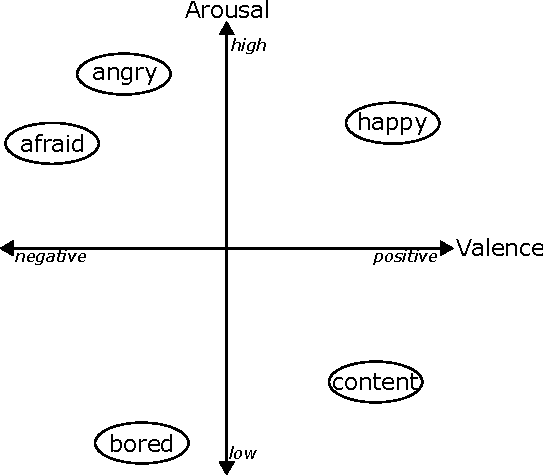
\includegraphics[scale=0.9]{2DemotionMapping.pdf}
	\caption{A two-dimensional emotion space with an Arousal and a Valence axis. Basic emotions are marked as ellipses within the quadrant. Adapted from \cite{vogt2008automatic}.}
	\label{fig:2.1 2-dimensional emotion space}
\end{figure}

\subsubsection{Applications}
Generally, there is a wide range of  applications in which emotion-aware speech recognition systems may be of use. 
For instance, in a call center, such an application could sort the incoming voice messages according to the emotion conveyed by the caller and could hence select the appropriate conciliation strategy.
Furthermore, the automobile industry is researching how the emotional state is influencing the driving behavior \cite{vogt2008automatic} and may develop corresponding driving assistants. 
Lastly, real-time emotion recognition in HCI-applications, for instance in the context of a nursing robot, needs yet to be mastered. 
In this context, the term 'emotion' may thus be interpreted in various ways and would hence comprise all sorts of human affects that may occur in HCI. 
Nevertheless, the more realistic the data becomes, the less feasible it is to classify emotions and human affect states correctly \cite{vogt2008automatic}. 
Figure \ref{fig:2.2 different Databases} shows how the difficulty of emotion recognition correlates with the dataset being used.
\begin{figure}[ht!]
	\centering
	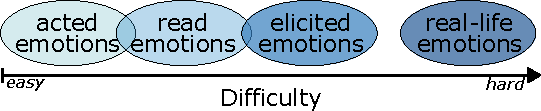
\includegraphics[scale=1.0]{differentDatabases.pdf}
	\caption{Types of databases used for emotion recognition and their difficulty. Adapted from \cite{vogt2008automatic}.}
	\label{fig:2.2 different Databases}
\end{figure}
\subsubsection{Automatic Speech Emotion Recognition System}
 As depicted in figure \ref{fig:2.3 speech emotion recognition system}, 
  a speech emotion recognition system consists of three principal parts: signal processing, feature extraction, and classification.
  Signal processing involves acoustic preprocessing, such as filtering the samples, as well as potentially segmenting them into meaningful units.
  Feature extraction is concerned with  identifying the relevant features of the acoustic signal  that are representative for emotions.
   Lastly, classification maps feature vectors onto emotion classes  through learning by examples \cite{vogt2008automatic}.
 
\begin{figure}[ht!]
	\centering
	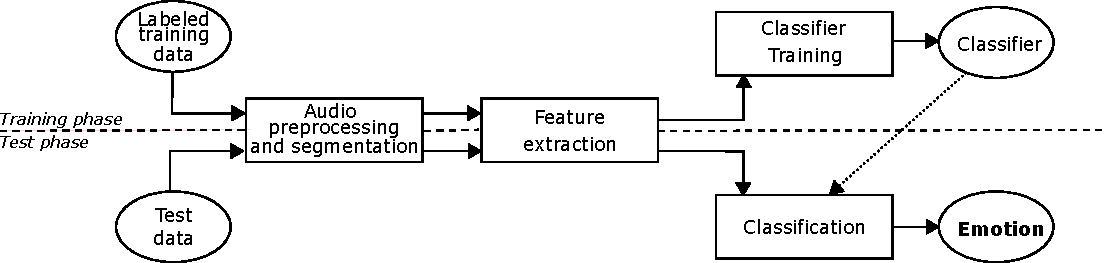
\includegraphics[width=\textwidth]{EmotionRecognitionSystem.pdf}
	\caption{Overview of speech emotion recognition system. Adapted from \cite{vogt2008automatic}.}
	\label{fig:2.3 speech emotion recognition system}
\end{figure}


\section{Data Processing}

\subsection{Signal Processing}
\subsubsection{Audio Segmentation}
Sound is transmitted in one-dimensional sound waves which have a single value based on the wave's height at every moment in time.
Next, sampling needs to be done which is the process of turning the sound wave into bits by recording the height of the wave at equally-spaced points.
While for 'CD Quality' audio is sampled at  44.1 kHz, a sampling of 16 kHz is enough for speech recognition in order to cover the frequency range of human speech. 
According to the \textit{Nyquist criterion}, the original sound wave can be reconstructed from the sampled one, as long as it is sampled at least twice as fast as the highest frequency aimed for to be recorded \cite{kester2009nyquist}. For this reason, no information is lost when sampling.


\subsection{The RAVDESS Dataset}
In this work, the \textit{Ryerson Audio-Visual Database of Emotional Speech and Song} (RAVDESS) is used. It is free of charge and can be downloaded at \texttt{\url{https://zenodo.org/record/1188976}}. 
The RAVDESS database 'is a validated multimodal database of speech and song [...]' \\ \cite{livingstone2018ryerson}. 24 professional actors and actresses, equally balanced in gender, were recorded phrasing main clauses such as  'Dogs are sitting by the door.' in North American English in one of the following eight emotions: neutral, calm, happy, sad, angry, fearful, disgust, surprised. Each of the 7356 RAVDESS files corresponds to a unique file name of which only the 1440 (= 60 trials per actor x 24) audio-only speech files are used in this work.

\subsection{Investigating the Data}
First, the raw audio waves as .wav data are loaded into the python script. 
As mentioned in section \ref{2.3.1.1 Audio Preprocessing}, this data could now be fed into the neural network, but speech or emotion recognition turns out to be difficult on raw audio waves.
Thus, some more preprocessing is done.  
Thereby, two problems have arisen, namely the variable length of the raw audio data, since CNNs require input samples of equal dimensions and the fact that the recordings consist of  unnecessary and meaningless silence  before and after the actual recorded speech as depicted in figure \ref{fig:untrimmed sw}. 
Hence, the audio samples are cropped in order to get rid of the meaningless silence.
However, the trimmed audio files  still are of different lengths, as shown in figure \ref{fig:trimmed sw}. 
This particular problem is solved differently for the two approaches and is thus elaborated on in more detail in the respective sections.

The raw audio wave data is  transformed into a spectrogram  as described in section \ref{2.3.1.1 Audio Preprocessing}. 
Figure\ref{fig:trimmed spec} depicts the corresponding spectrogram to the raw audio wave shown in figure \ref{fig:untrimmed sw} and figure \ref{fig:trimmed spec} depicts the respective spectrogram on the trimmed audio wave.


\subsubsection{Audio Preprocessing}
\label{2.3.1.1 Audio Preprocessing}
Arrays of numbers represent the amplitude of the sound wave at $\frac{1}{16000}$th of a second interval. 
This data could now be fed into a neural network, but recognizing speech or emotion patterns by processing these samples turns out to be difficult \cite{geitgey2016}. 
Instead, some more preprocessing on the audio data can be done by breaking apart the complex sound into its component parts by applying the Fourier Transform which breaks apart the complex sound wave into the simple sound waves that it is made up of \cite{Goodfellow-et-al-2016}.
Essentially, the sound wave is now split into its frequency parts. By adding up the energy that is contained in each frequency band, a quantification of the relevance of each frequency is obtained at every point in time. 
This representation is called a \textit{spectrogram} which is a suitable input representation of audio data for a neural network whereby the intensity of the spectral coefficients  is plotted versus the time index.

% the frequency energy encoded in color is depicted over time which is chunked into 20 ms intervals.
 
%\subsection{Fourier Transformation}


% \begin{figure}[ht!]
% 	\centering
% 	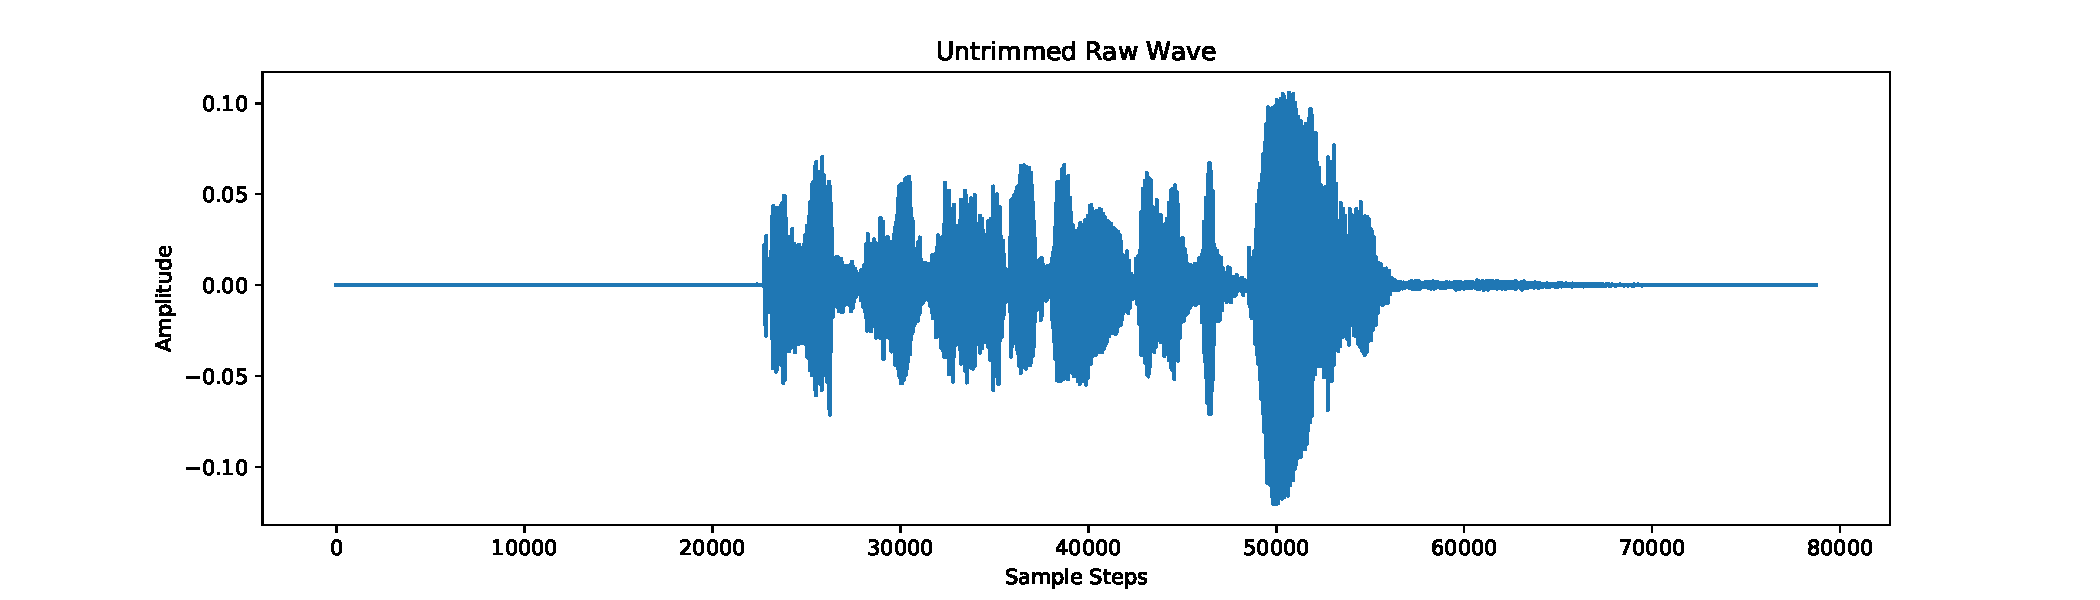
\includegraphics[scale=0.5]{untr_raw_wave.pdf}
% 	\caption{Un-trimmed sound wave of woman saying 'Dogs are sitting by the door.' in an fearful manner. There is still a lot of meaningless silence before and after the woman speaking. }
% 	\label{fig:untrimmed sw}
% \end{figure}
% \begin{figure}[ht!]
% 	\centering
% 	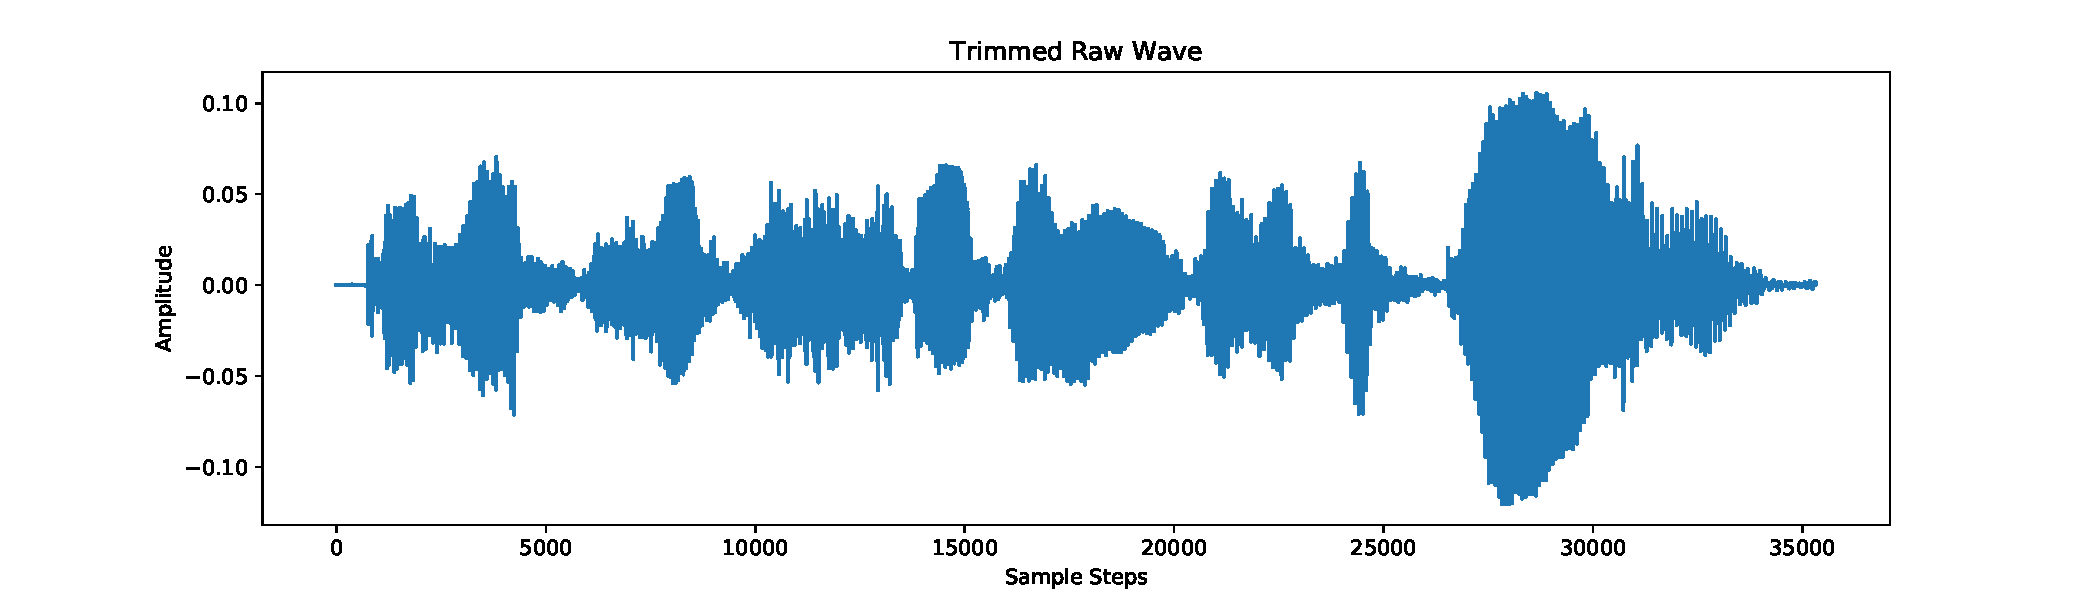
\includegraphics[scale=0.5]{tr_raw_wave.pdf}
% 	\caption{Corresponding trimmed raw wave which now only contains the recorded speech since the silence was trimmed.}
% 	\label{fig:trimmed sw}
% \end{figure}
% \begin{figure}[ht!]
% 	\centering
% 	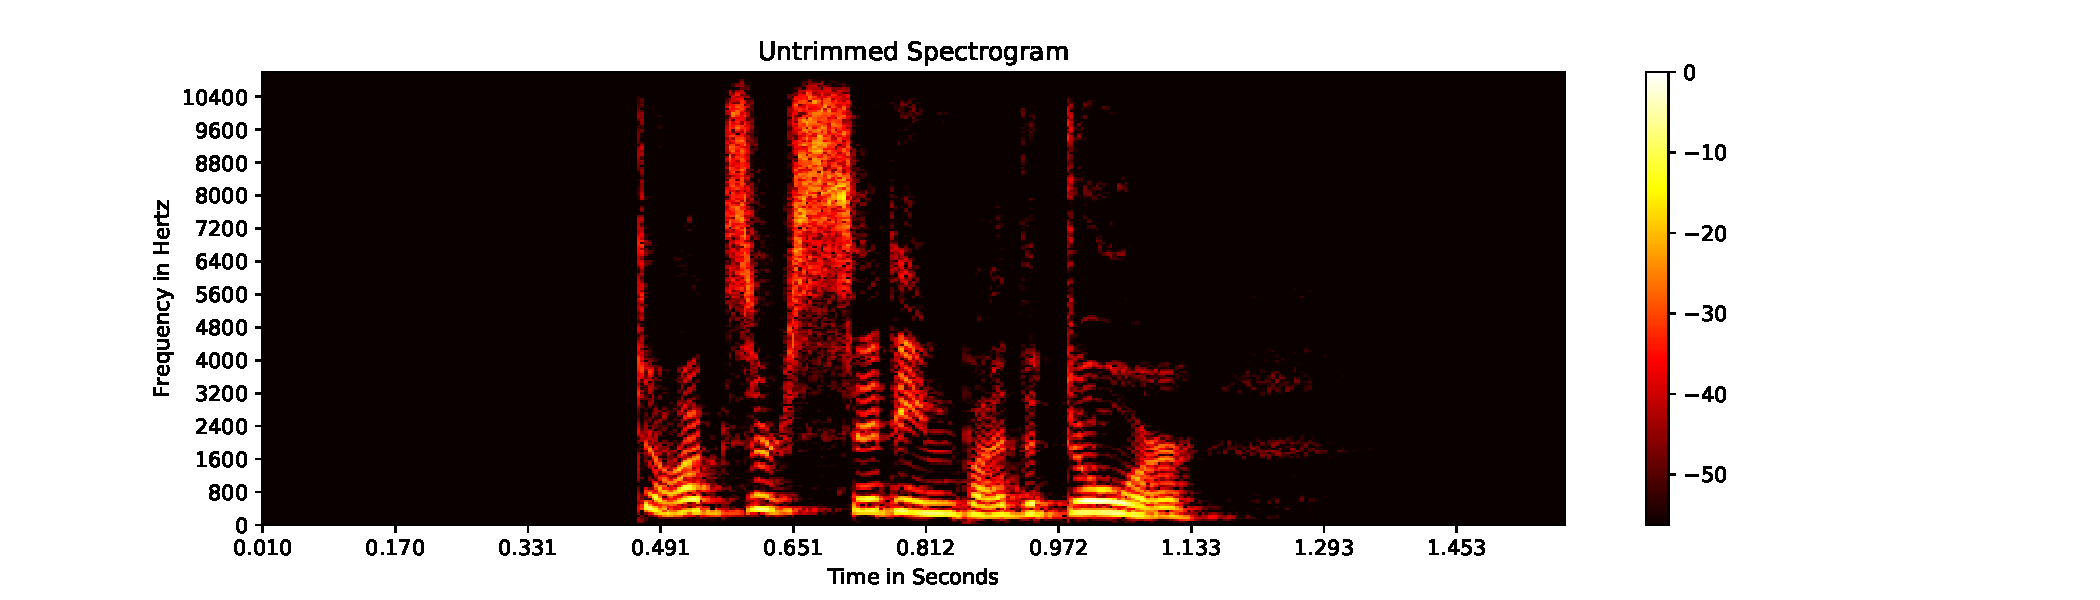
\includegraphics[scale=0.6]{untr_spectrogram.pdf}
% 	\caption{Corresponding spectrogram of un-trimmed raw wave of woman saying 'Dogs are sitting by the door.' in a angry manner.}
% 		\label{fig:untrimmed spec}
% \end{figure}
% \begin{figure}[ht!]
% 	\centering
% 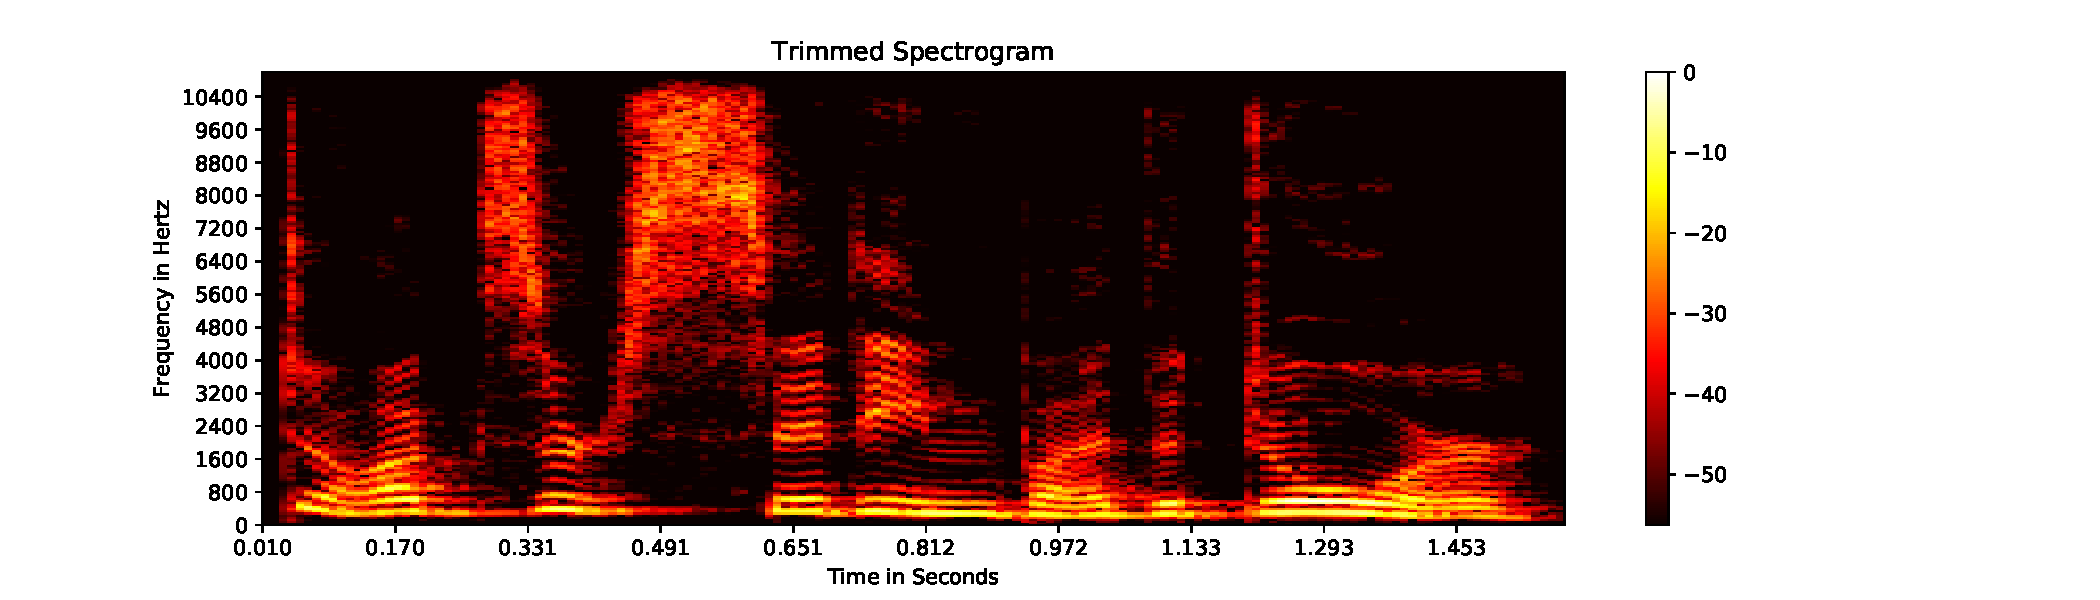
\includegraphics[scale=0.6]{tr_spectrogram.pdf}
% 	\caption{Respective spectrogram of trimmed raw wave.}
% 	\label{fig:trimmed spec}
% \end{figure}


\section{Methods}

% \subsection{Machine Learning}
% Machine Learning is concerned with relating a certain type of input to an output. That is, learning a specific function which represents the  dependencies between input and output values.
% Knowing such a functional relationship is of interest in a plethora of real-life applications, such as the following \cite{Smola2004} :
% \begin{itemize}
% 	\item make a diagnosis based on clinical measurements
% 	\item predict whether a client will pay back a loan to the bank
% 	\item assign the ASCII code to digitalized images of handwritten characters
% 	\item speech and emotion recognition
% 	\item estimate the costs of claims of insurees based on insurance data 
% \end{itemize}
% Preliminarily, in statistical learning theory or machine learning tasks, it is assumed to have gathered a finite set of input values with corresponding output values. 
% For instance, in the scenario above, data could have been collected on patients who already developed the disease \cite{Smola2004}.
% Thereby, the crucial goal is to find a prediction rule for output values that works well on new, at this point in time, unseen input data.

% More formally, a  probability distribution $P$ over the space $\mathcal{X} \times \mathcal{Y}$ is considered from which   data-label pairs $(X_i, Y_i)_{i=1...n}$ are sampled. 
% The goal is to approximate the best  possible classifier by a learned function $f_n: \mathcal{X} \rightarrow \mathcal{Y}$ based on this finite sample set which models the underlying distribution $P$. Note hereby, that during the training, $P$ is unknown. 
% In this specific case, the label space $\mathcal{Y}$ is discrete and consists of the eight categories which correspond to the eight emotions considered in the dataset used in this work. 

% Principally, any statistical classifier that is capable of dealing with high-dimensional  data is now a plausible choice for $f_n$.

In this project, two approaches are investigated: first, a \textit{Convolutional Neural Network} (CNN) (see section \ref{CNN}) and  second, a \textit{Support Vector Machine } (SVM). 
Having computed the spectrograms from the audio data, we now have appropriate features available that can be processed by a learning algorithm.
As the first approach, an CNN is trained on a spectrogram (see figure \ref{fig:trimmed spec}). 
However, neural networks require a large number of data which should exceed the 1440 samples of our data set by orders of magnitude. Thus, a second approach using a support vector machine is investigated since SVMs can handle small data sets well. 


% The implementation of the CNN is completely based on the open source machine learning environment TensorFlow \cite{tensorFlow}.
% For the SVM, the  Python module \textit{Scikit-learn} is \\used \cite{scikit-learn}.

For both approaches,  10\% of the data set is used as independent test set to evaluate the  model's ability to generalize.

Below, a very brief overview of CNNs and SVMs  is given from a high-level perspective.


\subsection{Approach 1: Convolutional Neural Networks}
\label{CNN}
\subsubsection{Foundations CNN}
Whilst being inspired by the concept of the mammalian retina, Convolutional Neural Networks (CNN) have been proven to be outstandingly effective on high-dimensional input \\
data \cite{Goodfellow-et-al-2016}. 
CNNs are a special kind of neural network, which use convolution as a specialized kind of linear operation in place of a general matrix multiplication  \cite{Goodfellow-et-al-2016}.
Advantageous to CNNs is their high efficiency in terms of  computational complexity while using a sparse set of parameters \cite{Goodfellow-et-al-2016}. 
The kernels which the CNN learns during training process, are reused over the entire input which markedly exceeds regular feed forward networks in terms of memory and computational efficiency.
For further details on the topic, the reader is referred to \cite{Goodfellow-et-al-2016}.


\subsubsection{Implementation of CNN}
The audio data is processed with a Fourier Transform whereas the audio waveform can be transformed into a tensor of rank two, i.e. a matrix. 
In doing so, the rows of the matrix correspond to different frequencies and the columns relate to different points in time.
However, the spectrograms are still of different lengths which is why zero padding is used to transform all samples to equal lengths. 
Thereafter, a min-max scaling is applied which means that to every value, $x = \frac{(x-min)}{max-min}$ is applied which normalizes the data to a value range of $[0,1]$. Hereby, \textit{min} and \textit{max} are the respective minimum and maximum values over the entire dataset.

\subsubsection{Evaluation of CNN:}

Surprisingly, in contrast to the prior assumption, the chosen model seems to be too simple and does not manage to learn the problem from the data. 
In every experiment ran -- due to  the restricted computational power  of the notebook used -- the training error does not converge, but rather oscillates around a constant value. 
It is safe to assume that the considered models  are too small and thus not powerful enough to make sense of the data.
Sine the training error is already unsatisfying, the model is not evaluated on the test set. 


\subsection{Approach 2: Support Vector Machines}
\label{SVM}
Support Vector Machines (SVM) are a widely used classifier due to its flexibility in modeling diverse sources of data and its ability to deal with high-dimensional data \cite{ben2010user}.
The goal of SVM is to find a hyperplane of the form $\mathcal{H} = \left\lbrace x \in \mathbb{R}^d | \left\langle w,x\right\rangle + b =0 \right\rbrace $ such that it separates the data while maximizing the distance between the hyperplane and the closest data point. This distance is referred to as the margin (see figute \ref{fig:2.4 svm}). By maximizing the margin, the classifier is most robust to noise in new data \cite{bishop2006pattern}. 

% \begin{figure}[ht!]
% 	\centering
% 	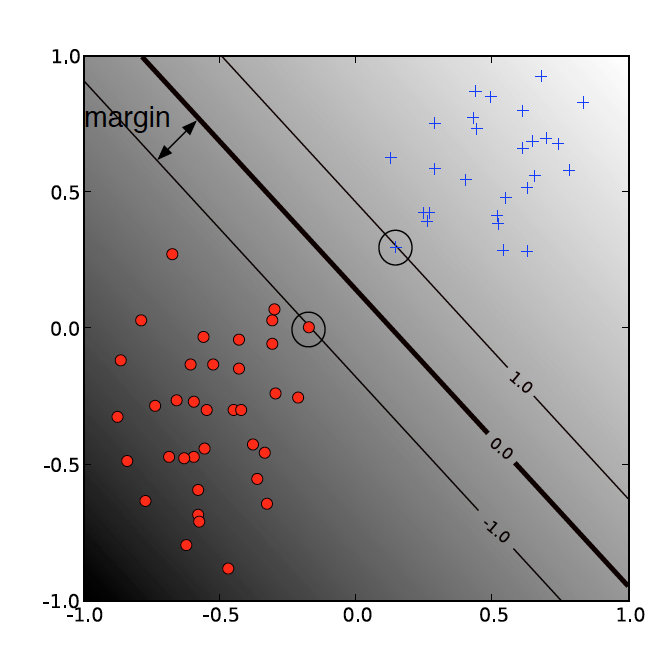
\includegraphics[scale=0.7]{svm.png}
% 	\caption{A linear SVM. The circled data points are the \textit{support vectors} -- i.e., the examples that are closest to the decision boundary. The support vectors determine the the margin with which the two classes are separated. In this work, eight classes need to be separated. From \cite{ben2010user}.}
% 	\label{fig:2.4 svm}
% \end{figure}

\subsubsection{Implementation of SVM:}

For the SVM, the  Python module \textit{Scikit-learn} is used \cite{scikit-learn}.
In order to feed the SVM a proper feature vector, the spectral coefficients from the spectrogram are  summed up over time.
While integrating over the time dimension, the temporal context is lost completely, however.

% \begin{figure}[ht!]
% 	\centering
% 	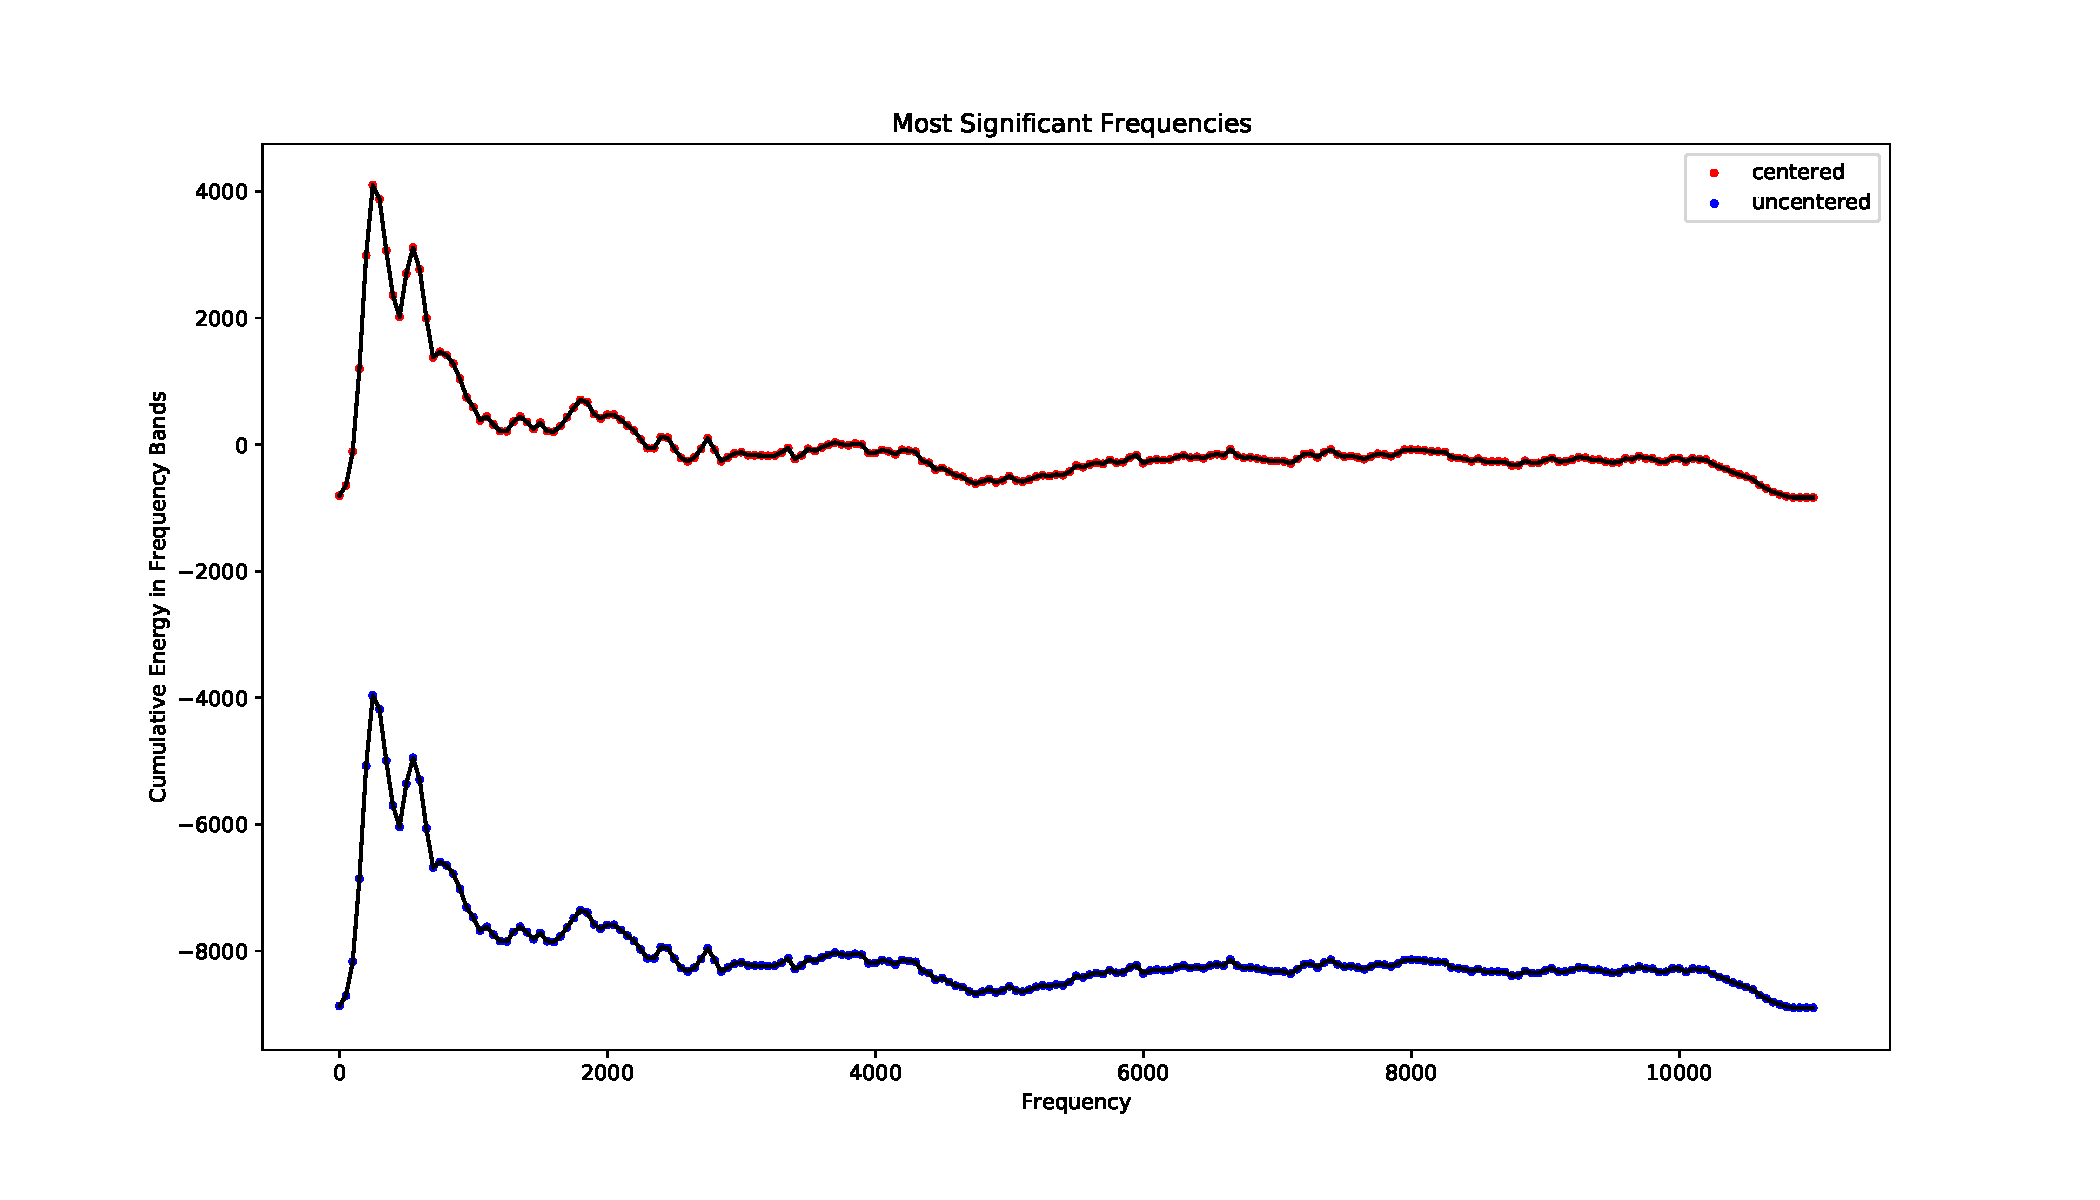
\includegraphics[width=\textwidth]{frequency_histogram.pdf}
% 	\caption{The cumulative sum of the frequencies in the respective  frequency bands as input for the SVM. }
% 	\label{fig:4.1 histogram}
% \end{figure}

Note that for this approach, no temporal dependencies in the audio data are taken into account, which seems counter-intuitive for speech processing at first glance. The model is expected to infer the emotions solely based on the frequency distribution as depicted in figure \ref{fig:4.1 histogram}. The figure shows both -- before and after centering -- the cumulative sum (y-axis) over each considered frequency band (x-axis) from the spectrogram. 
This results in a 'frequency-histogram' on which a dimension reduction algorithm, namely \textit{Principle Component Analysis }(PCA), is applied to reduce the dimensions of the input data  in order to obtain fewer, more meaningful features \cite{bishop2006pattern}. Thereby, the optimal parameters are obtained via Grid Search, both for PCA and SVM.
%The optimized hyper parameters include the kernel-width for both, PCA and SVM, as well as the soft-margin constant $C$ for the SVM and the number of principal components for the PCA.
%For further details regarding the impact of these parameters the reader is referred to \cite{bishop2006pattern, ben2010user}.
%As a brief overview it is important to mention that the algorithm is highly sensitive to the choice of the parameters and particularly to their combination. This impacts  the algorithm's ability to generalize to new data.
% From the Grid Search, the following values are   obtained as optimal parameters: \\\\
% \begin{align*}
% l = 745 \qquad &\text{(number of principal components of PCA)}\\
% \gamma_{\text{\tiny PCA}} =  1 \qquad &\text{(inversed kernel width of PCA)}\\
% C = 10 \qquad &\text{(soft-margin constant of SVM)}\\
% \gamma_{\text{\tiny SVM}} = 10 \qquad &\text{(inversed kernel width of SVM)}
% \end{align*}
% Note hereby, that the PCA is applied in an \textit{n}-dimensional feature space where $n$ is the number of samples, and therefore resulted in a dimension higher than the data dimension. Further details on this topic are beyond the scope of this work but can be looked up in \cite{steinwart2008support}.
% Furthermore, it is noteworthy, that there might exist better hyperparameters than the ones Grid Search has determined in our case.


%s\subsubsection{Evaluation of SVM}
%For this approach, no temporal dependencies in the audio data are taken into account, which seems counter-intuitive for speech processing at first glance. The model is expected to infer the emotions solely based on the frequency distribution as depicted in figure \ref{fig:4.1 histogram}. The figure shows both -- before and after centering -- the cumulative sum (y-axis) over each considered frequency band (x-axis) from the spectrogram. This results in a 'frequency-histogram' on which a dimension reduction algorithm, namely \textit{Principle Component Analysis }(PCA), is applied to reduce the dimensions of the input data  in order to obtain fewer, more meaningful features \cite{bishop2006pattern}. Thereby, the optimal parameters are obtained via Grid Search, both for PCA and SVM.
%The optimized hyper-parameters include the kernel-width for both, PCA and SVM, as well as the soft-margin constant $C$ for the SVM and the number of principal components for the PCA.
%For further details regarding the impact of these parameters the reader is referred to \cite{bishop2006pattern, ben2010user}.
%As a brief overview it is important to mention that the algorithm is highly sensitive to the choice of the parameters and particularly to their combination. This impacts  the algorithm's ability to generalize to new data.
% From the Grid Search, the following values are   obtained as optimal parameters: \\\\
% \begin{align*}
% l = 745 \qquad &\text{(number of principal components of PCA)}\\
% \gamma_{\text{\tiny PCA}} =  1 \qquad &\text{(inversed kernel width of PCA)}\\
% C = 10 \qquad &\text{(soft-margin constant of SVM)}\\
% \gamma_{\text{\tiny SVM}} = 10 \qquad &\text{(inversed kernel width of SVM)}
% \end{align*}
% Note hereby, that the PCA is applied in an \textit{n}-dimensional feature space where $n$ is the number of samples, and therefore resulted in a dimension higher than the data dimension. Further details on this topic are beyond the scope of this work but can be looked up in \cite{steinwart2008support}.
% Furthermore, it is noteworthy, that there might exist better hyperparameters than the ones Grid Search has determined in our case.




%% Restructured and moved to Methods
%\section{Approach}






\section{Conclusion}
Two approaches have been investigated for the  task of automatic emotion recognition. 
The motivation was to use machine learning algorithms in order to infer emotions from recorded speech. 
Thereby, a Deep Learning approach was chosen first, whereby a Convolutional Neural Network (CNN) was trained on the RAVDESS data set. 
Regrettably, it did not learn the problem at all. Due to the small number of training samples and the lack of computational power, this approach was not further pursued but certainly remains an interesting topic to investigate within a larger scaled project. 
Therefore, the insights of the first attempt gave rise to a different approach, namely a  Support Vector Machine (SVM).
An SVM works well on smaller data sets and delivered surprisingly good results. An accuracy of 97.05\% on the training set and 63.89\% on the test set was achieved. 
This demonstrates that the SVM predicts emotions correctly way beyond chance and in addition, only based on most relevant frequencies related to the respective emotion since the temporal context is lost completely in this latter approach.
This suggests that this machine learning algorithm is able to predict emotions from recorded speech data only based on the respective, relevant frequencies. 
Consequently, one may conclude that emotions are encoded in specific frequencies to a large extent. 
Undoubtedly, these results are far from being able to be generally applicable for automatic emotion recognition, since  this task  becomes more difficult the more realistic the data set is, which is illustrated in figure \ref{fig:2.2 different Databases}.
Unfortunately, it is difficult to compare results on automatic emotion recognition among publications since most researchers use different speech data sets,  speaker types, and  classifiers. Additionally, in this field of research, there exists no consistent  benchmark, such as MNIST in the field of pattern recognition on images \cite{mnist}.

\subsection{Future Work}
Besides these already promising results, further investigation regarding the deep learning approach might be worthwhile. 
For instance, different neural networks such as Recurrent Neural Networks (RNN) \cite{DBLP:series/sci/2012-385} or a combination of different architectures might be interesting to  investigate. Additionally, a different padding to the spectrogram could be applied. 
Furthermore, different parameters could be tried with the SVM. 
Moreover, a dynamic classifier such as Hidden Markov Models (HMM) seems to work well. Such dynamic modelling techniques are also the most common ones found in literature on automatic emotion recognition on speech \cite{vogt2008automatic}.

Overall, this project shows, that SVMs are a promising technique for the task of automatic emotion recognition on speech data.

\newpage

\section{Appendix}\label[]{Appendix}
%%%%%%%%%%%%%%%%%%%%%%%%%%%%%%%%%%%%%%%%%%%%%%%%%%%%%%%%%%%%%%%%%%%%%%%%%%%%%%%%%%%%%%%%%%%%%%%%%%%%%%%%%%%%
%%%%%%%%%%%%%%%%%%%%%%%%%%%%%%%%%%%%%%%%%%%%%%%%%%%%%%%%%%%%%%%%%%%%%%%%%%%%%%%%%%%%%%%%%%%%%%%%%%%%%%%%%%%%
% \subsection{Background}
% \begin{table}
% 	%\tablepreamble
% 	\newcolumntype{Y}{>{\centering\arraybackslash}X}
% 	\renewcommand{\arraystretch}{1.1}
% 	\centering
% 	\caption[]{Some variations of acoustic variables observed in relation to emotions, from \cite{vogt2008automatic}.}
% 	\label{tbl:stats}
% 	\begin{tabularx}{\textwidth}{YYYYY}
% 		\toprule
% 		\textbf{Emotion}&  \textbf{Pitch} &  \textbf{Intensity} &  \textbf{Speaking Rate}&\textbf{Voice Qualtiy}  \\
% 		\midrule
% 		\rowcolor{tblhead}
% 		Anger & high mean, wide range& increased& increased &breathy; blaring timbre \\
% 		Joy & increased mean and range & increased &increased &sometimes breathy; moderately blaring timbre\\
% 		\rowcolor{tblhead}
% 		Sadness & normal or lower than normal mean, narrow range & decreased & slow& resonant timbre  \\
% 		\bottomrule
% 	\end{tabularx}
% \end{table}

\subsection{Figures of Data Processing}\label[]{sec:dataprocessing}
\subsubsection{For CNN}
\begin{figure}[ht!]
	\centering
	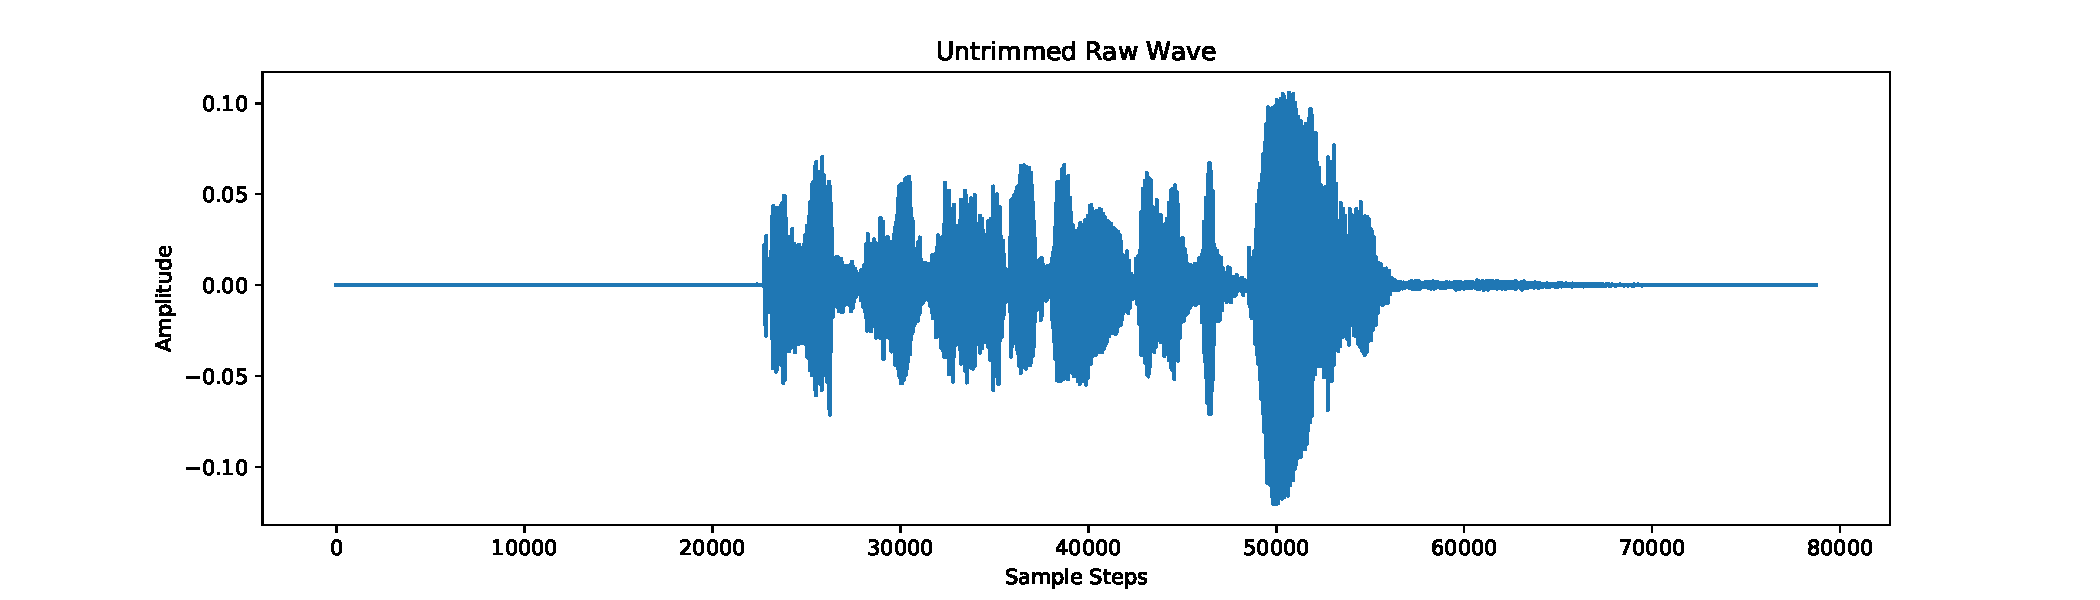
\includegraphics[scale=0.5]{untr_raw_wave.pdf}
	\caption{Un-trimmed sound wave of woman saying 'Dogs are sitting by the door.' in an fearful manner. There is still a lot of meaningless silence before and after the woman speaking. }
	\label{fig:untrimmed sw}
\end{figure}
\begin{figure}[ht!]
	\centering
	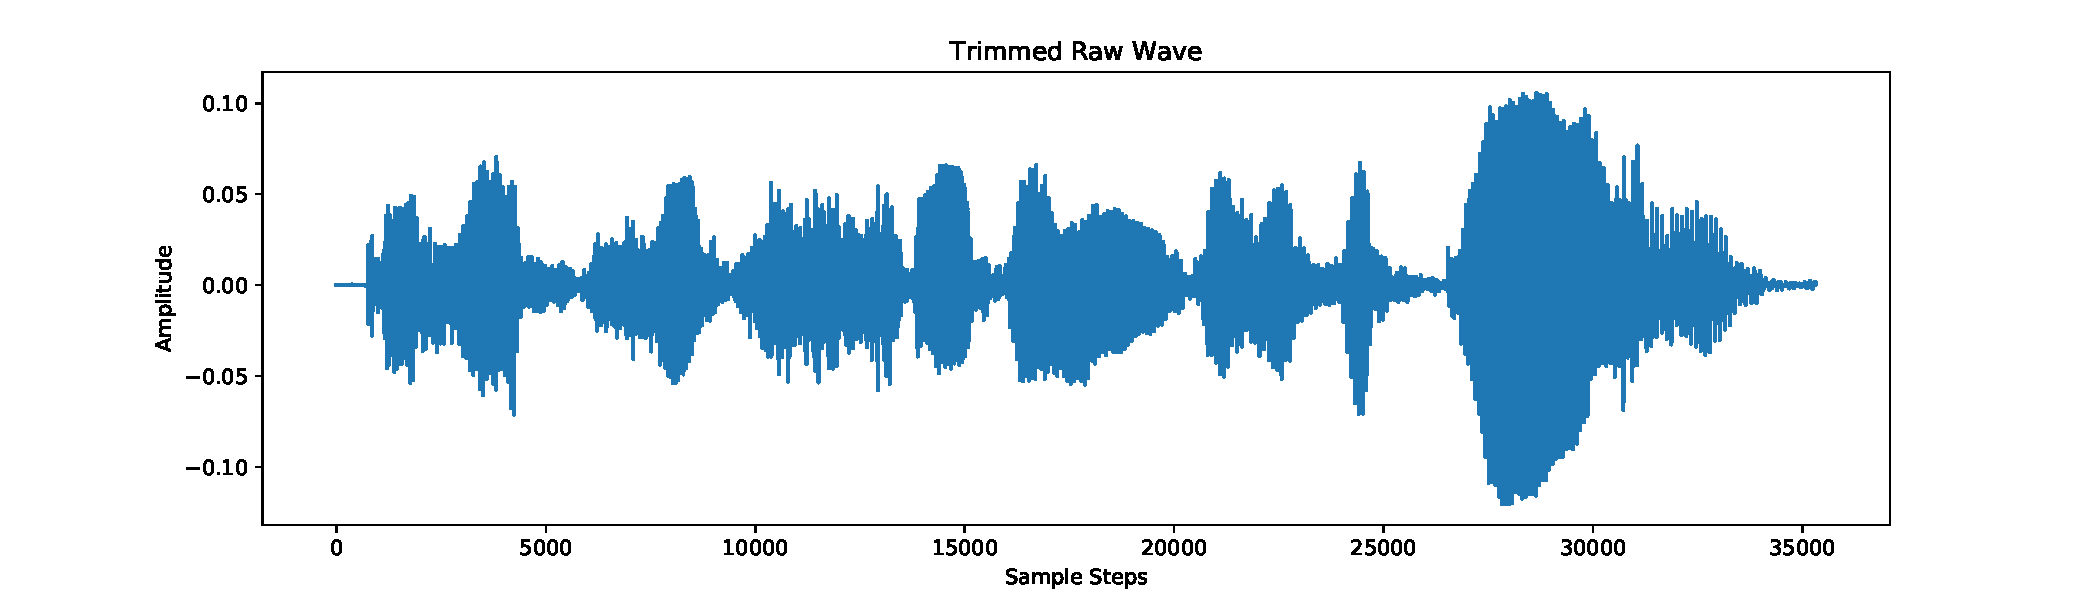
\includegraphics[scale=0.5]{tr_raw_wave.pdf}
	\caption{Corresponding trimmed raw wave which now only contains the recorded speech since the silence was trimmed.}
	\label{fig:trimmed sw}
\end{figure}
\begin{figure}[ht!]
	\centering
	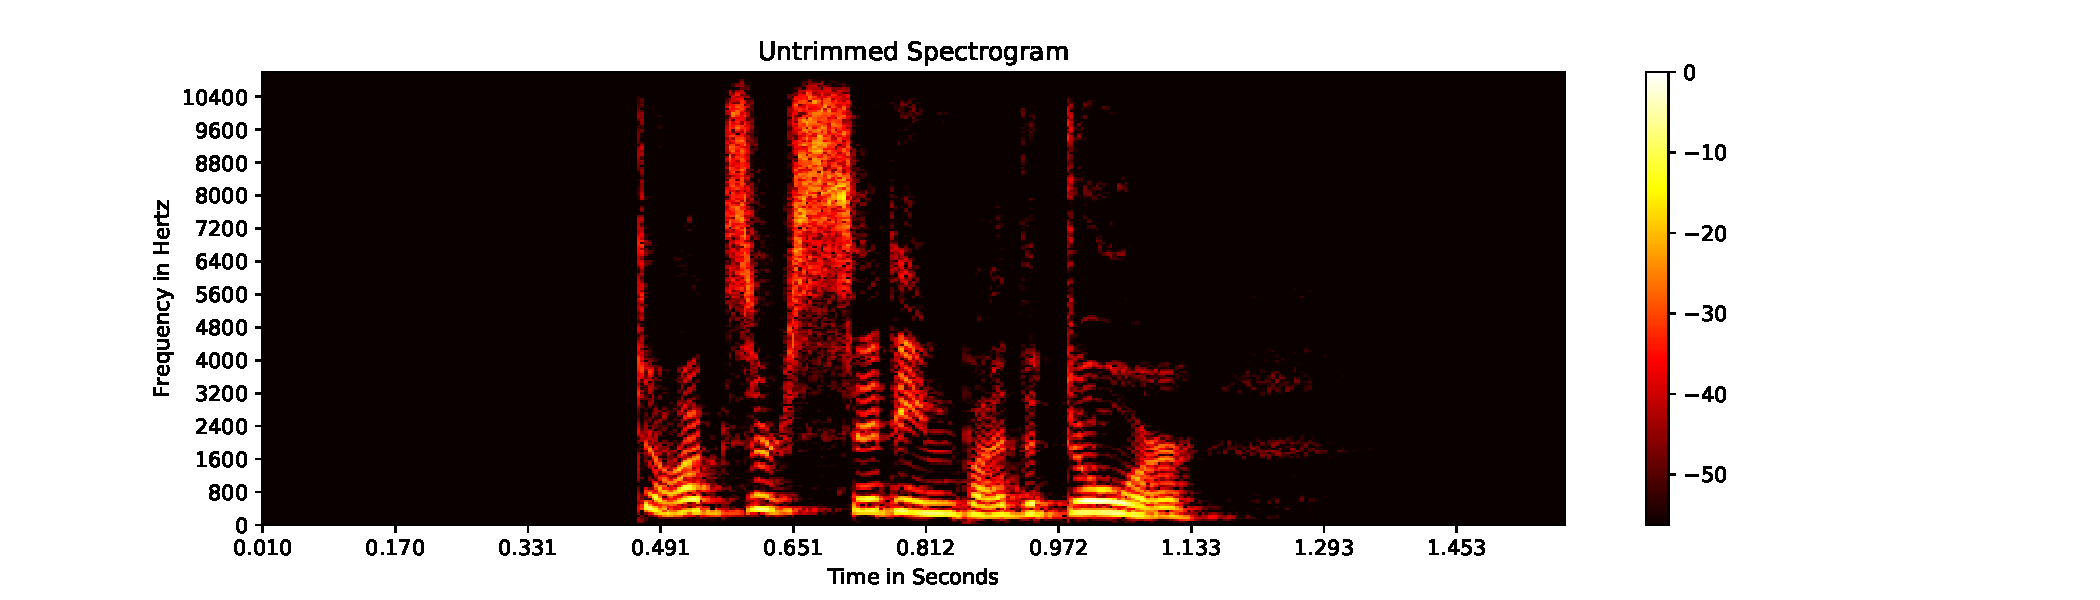
\includegraphics[scale=0.6]{untr_spectrogram.pdf}
	\caption{Corresponding spectrogram of un-trimmed raw wave of woman saying 'Dogs are sitting by the door.' in a angry manner.}
		\label{fig:untrimmed spec}
\end{figure}
\begin{figure}[ht!]
	\centering
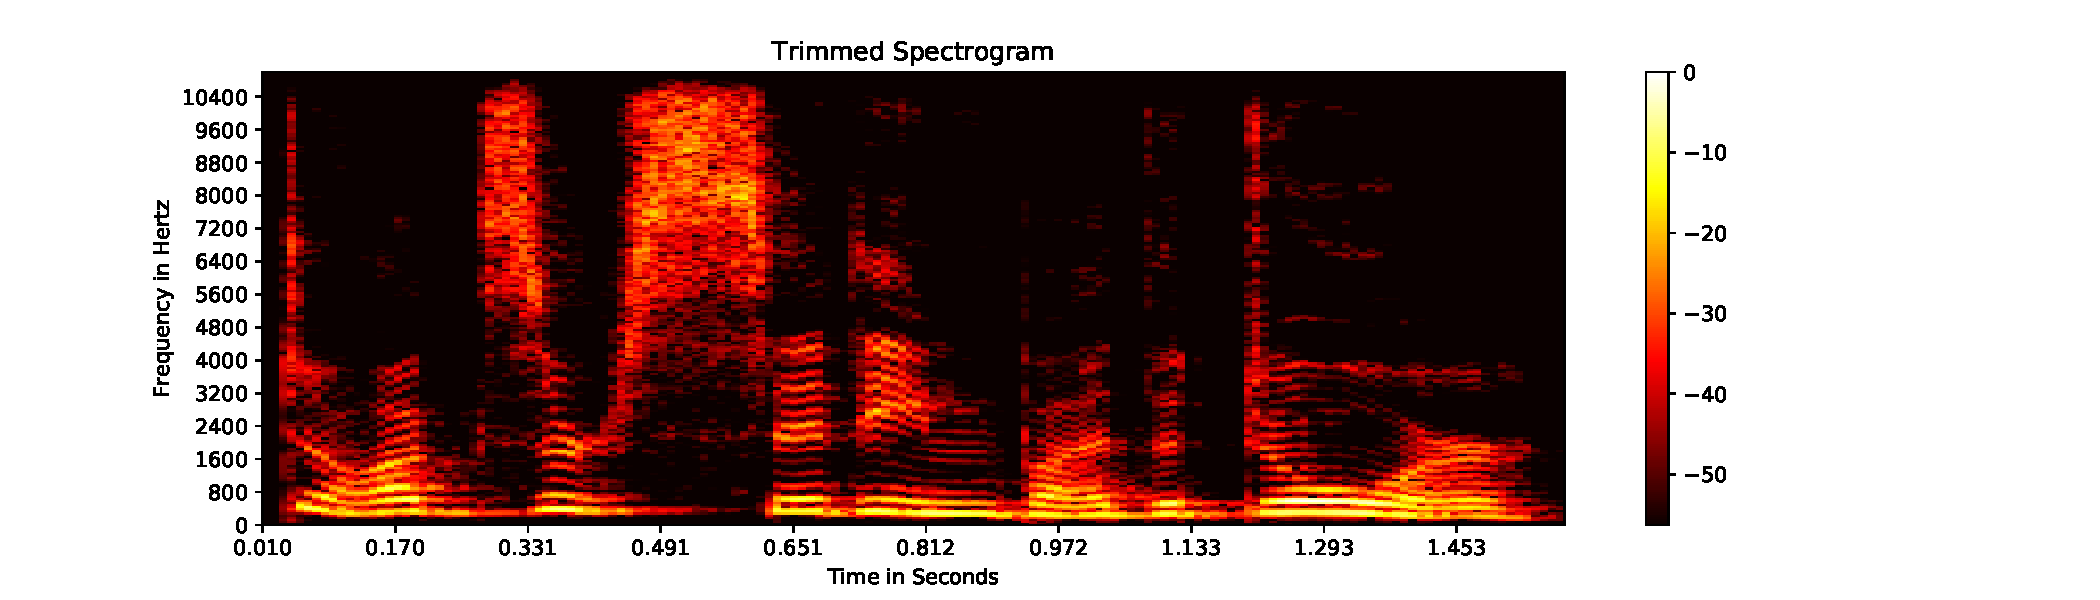
\includegraphics[scale=0.6]{tr_spectrogram.pdf}
	\caption{Respective spectrogram of trimmed raw wave.}
	\label{fig:trimmed spec}
\end{figure}

\newpage
%\subsubsection{For SVM:}

\begin{figure}[htp!]
	\centering
	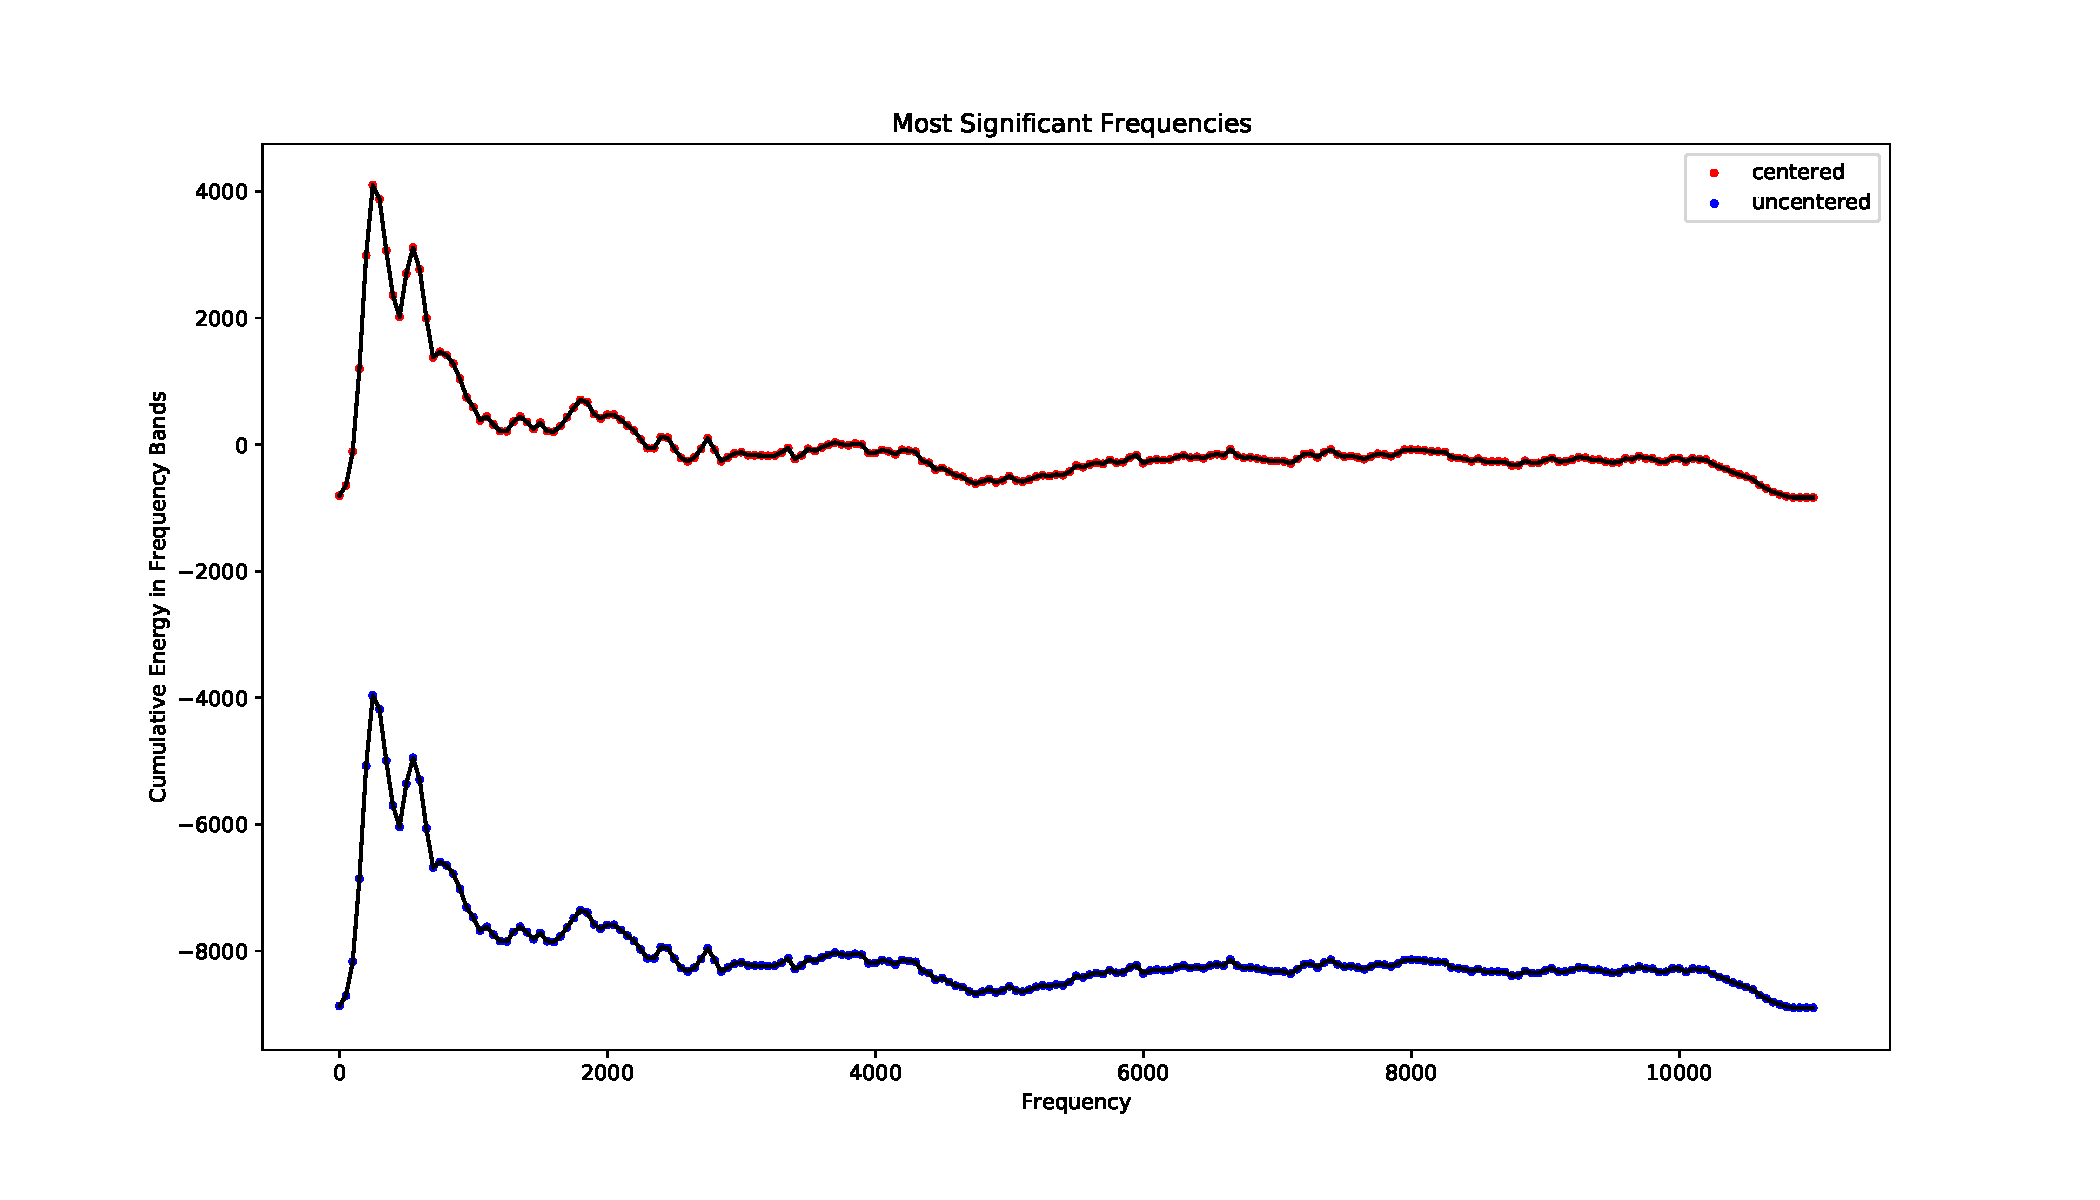
\includegraphics[scale=.5]{frequency_histogram.pdf}
	\caption{The cumulative sum of the frequencies in the respective  frequency bands as input for the SVM. }
	\label{fig:4.1 histogram}
\end{figure}




\subsection{Figures and Parameters for SVM-Model}

\begin{figure}[ht!]
	\centering
	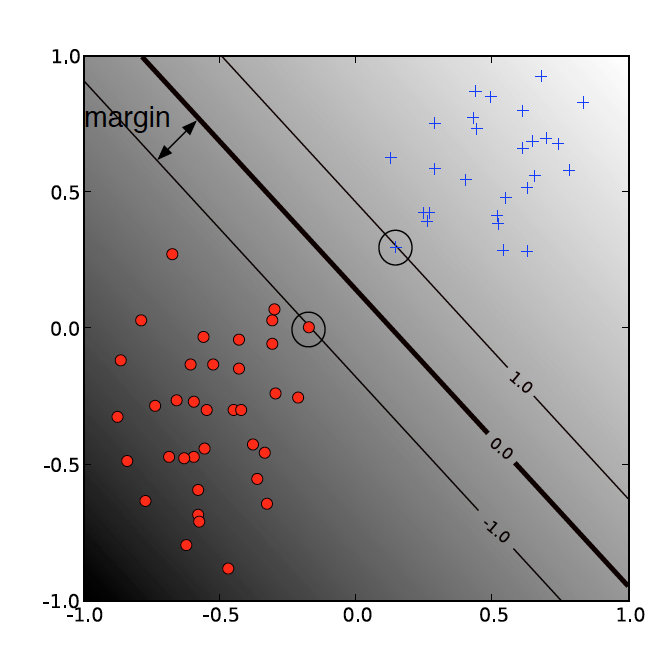
\includegraphics[scale=0.7]{svm.png}
	\caption{A linear SVM. The circled data points are the \textit{support vectors} -- i.e., the examples that are closest to the decision boundary. The support vectors determine the the margin with which the two classes are separated. In this work, eight classes need to be separated. From \cite{ben2010user}.}
	\label{fig:2.4 svm}
\end{figure}


\subsubsection{SVM Model Parameters}
From the Grid Search, the following values are   obtained as optimal parameters: \\\\
\begin{align*}
l = 745 \qquad &\text{(number of principal components of PCA)}\\
\gamma_{\text{\tiny PCA}} =  1 \qquad &\text{(inversed kernel width of PCA)}\\
C = 10 \qquad &\text{(soft-margin constant of SVM)}\\
\gamma_{\text{\tiny SVM}} = 10 \qquad &\text{(inversed kernel width of SVM)}
\end{align*}
Note hereby, that the PCA is applied in an \textit{n}-dimensional feature space where $n$ is the number of samples, and therefore resulted in a dimension higher than the data dimension. Further details on this topic are beyond the scope of this work but can be looked up in \cite{steinwart2008support}.
Furthermore, it is noteworthy, that there might exist better hyperparameters than the ones Grid Search has determined in our case.


%\newpage
%\listoffigures
%\listoftables
% \newpage
\newpage
\section{References}
{\small
\bibliographystyle{unsrtnat}
\bibliography{../literature/ref.bib}
}

\end{document}



